\section{Supplementary material}

\subsection{Selection of potential new MT units by net benefit}

We tested each IVT-only unit to estimate the potential gain from adding that unit as a single extra MT unit. The model predicted the catchment population of the new MT provision, as a sum of admissions to that unit and all surrounding IVT-only units where the new MT unit would be the closest (fast travel time) MT unit. The model also predicted the benefit to those patients. The total net benefit from adding each unit is the product of the catchment population and the benefit achieved to that population. Two units may have the same net benefit but one by having a smaller benefit over a larger population, and the other having a larger benefit over a smaller benefit. Table \ref{tab:hospital-benefit} shows the top 40 units as measured by the total net benefit. Figure \ref{fig:benefit_pareto} plots catchment population against benefit to that population, and the resulting net benefit.

\begin{table}[H]
\centering
\small
\caption{Estimated benefit by hospital location. Each hospital is tested as a single extra MT unit in addition to current provision. The \textit{Admission Catchment Benefitting} is the catchment of that extra MT unit and all the IVT-only units that would likely use the new MT unit. The \textit{Mean Benefit} is the number of additional good outcomes (mRS 0-2 at 3-6 months) for 100 patients treated with MT at the new MT unit. The \textit{Relative Benefit} is the product of the \textit{Admission Catchment Benefitting} and the \textit{Mean Benefit}, scaled to the maximum benefit observed. Results show the hospitals in the top 40 relative benefit.}
\label{tab:hospital-benefit}
\begin{tabular}{lrrr}
\toprule
Hospital Location & \shortstack[r]{Admission Catchment\\Benefiting} & \shortstack[r]{Mean\\Benefit} & \shortstack[r]{Relative\\Benefit} \\
\midrule
Harrow              & 6164 & 1.90 & 1.00 \\
Smethwick           & 6206 & 1.56 & 0.83 \\
Watford             & 4980 & 1.93 & 0.82 \\
Bournemouth         & 2090 & 4.24 & 0.76 \\
Stockport           & 1743 & 4.88 & 0.73 \\
Northampton         & 3458 & 2.42 & 0.72 \\
Frimley Park        & 2705 & 3.09 & 0.72 \\
Taunton             & 2736 & 2.95 & 0.69 \\
Wolverhampton       & 3279 & 2.44 & 0.69 \\
Dartford            & 2879 & 2.57 & 0.63 \\
Peterborough        & 1716 & 4.27 & 0.63 \\
Reading             & 4245 & 1.71 & 0.62 \\
Portsmouth          & 1980 & 3.62 & 0.61 \\
Chertsey            & 3320 & 2.16 & 0.61 \\
Luton and Dunstable & 4456 & 1.58 & 0.60 \\
Exeter              & 2680 & 2.60 & 0.60 \\
Bury                & 1417 & 4.88 & 0.59 \\
Doncaster           & 2769 & 2.48 & 0.59 \\
Leicester           & 2273 & 2.95 & 0.57 \\
Truro               &  834 & 7.95 & 0.57 \\
Milton Keynes       & 2420 & 2.73 & 0.57 \\
Colchester          & 1332 & 4.94 & 0.56 \\
High Wycombe        & 5329 & 1.17 & 0.54 \\
Dudley              & 3221 & 1.93 & 0.53 \\
Lincoln             &  917 & 6.78 & 0.53 \\
York                & 1021 & 6.06 & 0.53 \\
Stevenage           & 3367 & 1.84 & 0.53 \\
Maidstone           & 1078 & 5.60 & 0.52 \\
Telford             &  931 & 6.24 & 0.50 \\
Cheltenham          & 2762 & 2.10 & 0.50 \\
Bradford            & 1694 & 3.33 & 0.48 \\
Derby               & 1099 & 5.11 & 0.48 \\
Torbay              & 2682 & 2.08 & 0.48 \\
Basildon            & 3784 & 1.44 & 0.47 \\
Epsom               & 3270 & 1.67 & 0.47 \\
Ipswich             & 1700 & 3.20 & 0.47 \\
Worcester           & 2010 & 2.69 & 0.46 \\
Dorchester          &  729 & 7.34 & 0.46 \\
Swindon             & 2334 & 2.29 & 0.46 \\
Carlisle            &  683 & 7.81 & 0.46 \\
\bottomrule
\end{tabular}
\end{table}

\begin{figure}[H]
    \centering
    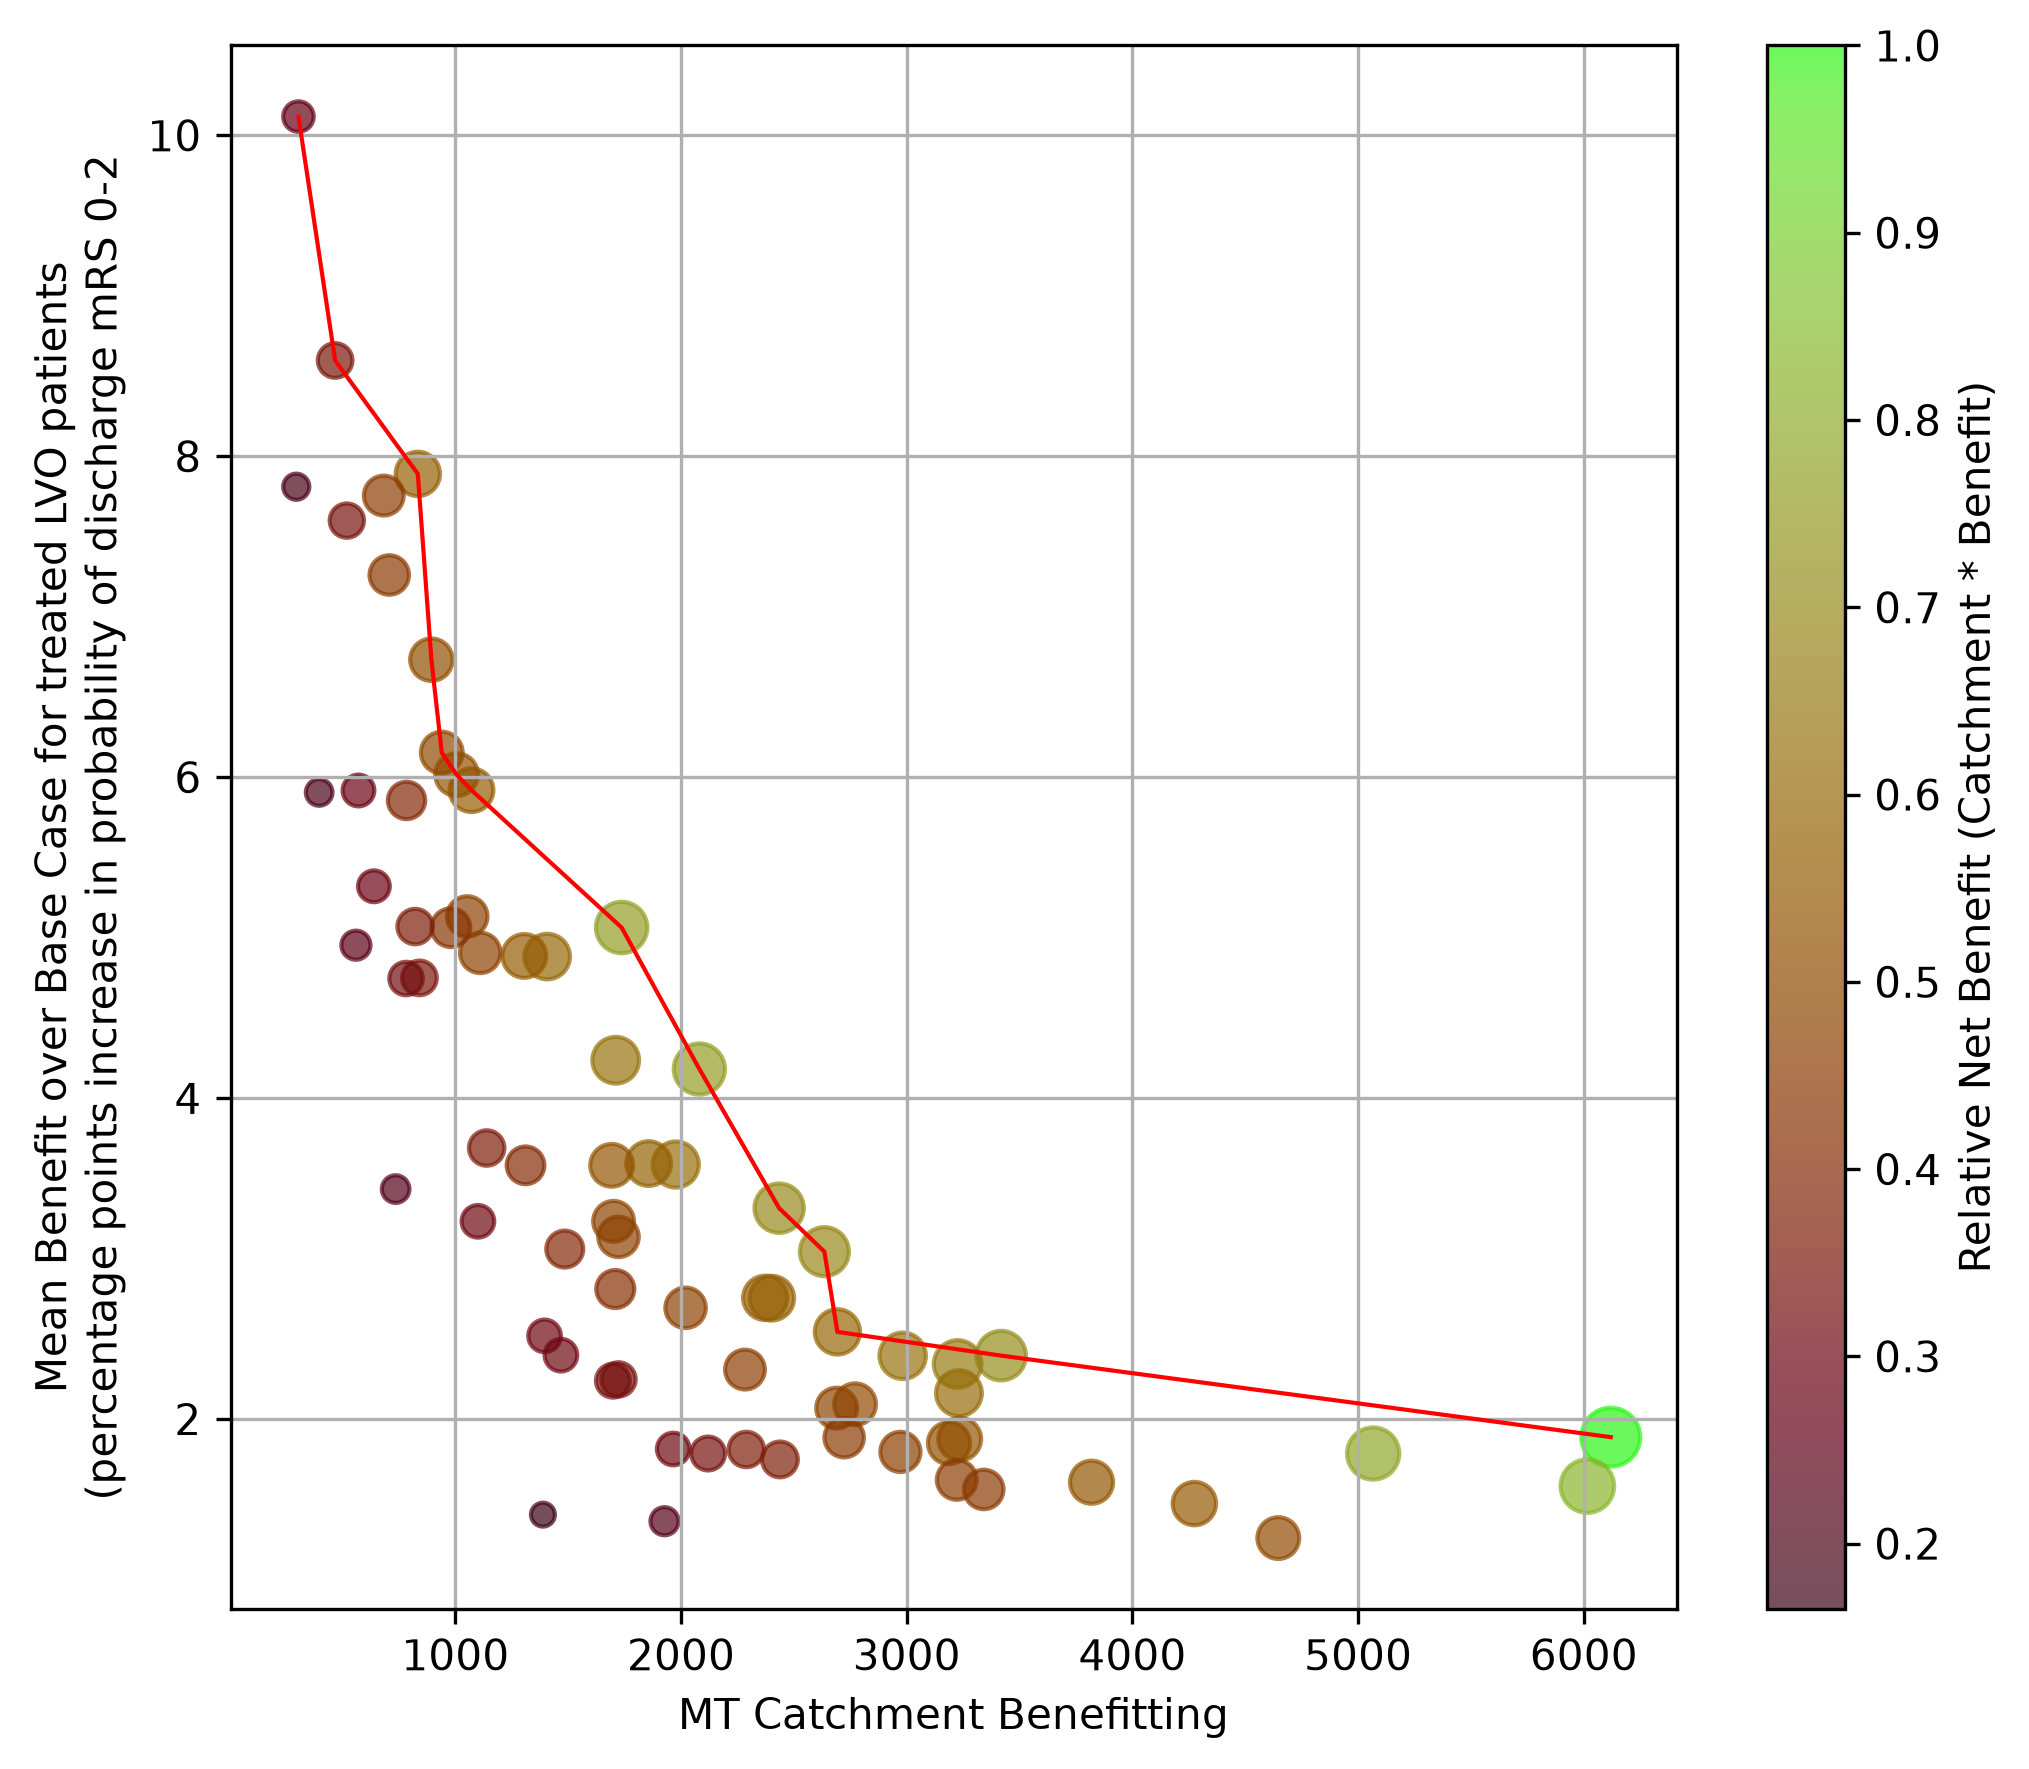
\includegraphics[width=0.66\linewidth]{images/mt_unit_benefit_plot.png}
    \caption{The benefit of adding a single new MT unit, chosen from current IVT-only units. The \textit{x-axis} shows catchment area (emergency stroke admissions per year) that would be redirected to the new MT unit. The \textit{y-axis} shows the benefit that redirected LVO patients would have if treated at the new MT unit (rather than at their current closest MT unit). Each point is sized and coloured by the net benefit (the product of the catchment area and the potential benefit for each person). The red line shows the \textit{Pareto front} where no other unit has both a larger catchment and a better benefit per person.}
    \label{fig:benefit_pareto}
\end{figure}

\subsection{MT units admission numbers}

Table~\ref{tab:mt_units_all} shows the numbers of MT admissions including patients transferred from other units for all MT units in England.

\begin{landscape}
\begin{table}[htbp]
    \centering
    \caption{Current and planned mechanical thrombectomy (MT) activity by MT unit, including additional MT units at Taunton and Worcester (``Planned MT''). All numbers assume 10\% of all stroke receive MT. 100\% transfer assuming there was no loss of chance to receive MT by first attending an IVT-only unit, and 67\% transfer assumes that 67\% of patients receive MT when first attending an IVT-only unit.}
    \label{tab:mt_units_all}
    \begin{tabular}{ll|rrr|rrr}
    \hline
     &  & & 100\% transfer & & & 67\% transfer & \\
    SSNAP Region & MT Unit & Current MT & Planned MT & Change & Current MT & Planned MT & Change \\
    \hline
    Buckinghamshire, Oxford and Berkshire & Oxford & 310 & 310 & 0 & 234 & 234 & 0 \\
    Cheshire and Mersey & Aintree & 400 & 400 & 0 & 320 & 320 & 0 \\
    East Midlands & Nottingham & 408 & 408 & 0 & 319 & 319 & 0 \\
    East of England (North) & Cambridge & 300 & 300 & 0 & 224 & 224 & 0 \\
    East of England (North) & Norwich & 302 & 302 & 0 & 243 & 243 & 0 \\
    Greater Manchester & Salford & 528 & 528 & 0 & 425 & 425 & 0 \\
    Humber Coast and Vale & Hull & 182 & 182 & 0 & 158 & 158 & 0 \\
    Kent and Medway & Canterbury & 222 & 222 & 0 & 187 & 187 & 0 \\
    Lancashire and South Cumbria & Preston & 288 & 288 & 0 & 218 & 218 & 0 \\
    London & Charing Cross & 452 & 452 & 0 & 333 & 333 & 0 \\
    London & Kings College & \textbf{100} & \textbf{100} & 0 & \textbf{100} & \textbf{100} & 0 \\
    London & Romford & 542 & 542 & 0 & 419 & 419 & 0 \\
    London & Royal London & \textbf{132} & \textbf{132} & 0 & \textbf{132} & \textbf{132} & 0 \\
    London & St George’s & 392 & 392 & 0 & 291 & 291 & 0 \\
    London & UCL & 281 & 281 & 0 & 227 & 227 & 0 \\
    North East and North Cumbria & Middlesbrough & 164 & 164 & 0 & \textbf{137} & \textbf{137} & 0 \\
    North East and North Cumbria & Newcastle & 478 & 478 & 0 & 369 & 369 & 0 \\
    North Midlands & Stoke & 173 & 173 & 0 & 152 & 152 & 0 \\
    South Yorkshire and Bassetlaw & Sheffield & 308 & 308 & 0 & 250 & 250 & 0 \\
    Sussex & Brighton & 202 & 202 & 0 & 157 & 157 & 0 \\
    SW Peninsula & Plymouth & 341 & 232 & -109 & 256 & 182 & -73 \\
    Wessex & Southampton & 560 & 491 & -69 & 402 & 356 & -46 \\
    West Midlands & Birmingham & 711 & 589 & -122 & 505 & 423 & -82 \\
    West Midlands & Coventry & 384 & 384 & 0 & 307 & 307 & 0 \\
    West Midlands & Worcester & 0 & 202 & 202 & 0 & 159 & 159 \\
    West of England & North Bristol & 394 & 220 & -174 & 308 & 192 & -116 \\
    West of England & Taunton & 0 & 272 & 272 & 0 & 214 & 214 \\
    West Yorkshire and Harrogate & Leeds & 522 & 522 & 0 & 397 & 397 & 0 \\
    \hline
    \end{tabular}
\end{table}
\end{landscape}


\subsection{Target trial emulation on timing of thrombolysis and thrombectomy}

In the SAMueL (Stroke Audit Machine Learning) project we performed a target trial on patients identified as having an LVO, or a stroke severity (NIHSS) of 11+. To emulate a clinical trial, we constructed comparable treatment and control groups by finding a matched untreated patient for each treated patient. Patients were matched on features found to significantly affect outcome or probability of receiving thrombolysis or thrombectomy, namely prior disability, age group (5 year bands), stroke severity bands (NIHSS 0-4, 5-9, 10-14, \textit{et seq.}), atrial fibrillation anti-coagulant, and atrial fibrillation diagnosis. Treated patients were assigned to one of 7 treatment groups, based on the treatment received (IVT only, MT only, or both), and the time that treatment is received (early is within 270 minutes from stroke onset, or late is beyond 270 minutes from stroke onset). When both treatments are given, IVT is received before MT. Non-matched treated patients were dropped from the analysis to ensure common support between control and test groups (the maximum dropped was 2.3\% of any treatment group).

Each treatment group had its own untreated control matched group. Discharge with disability was then compared between control and treated patients in each treatment group. 

Figure \ref{fig:main_target_trial_mrs_2} shows the differences between control and treated groups for each of the 7 treatment groups (early or late IVT and/or MT). Early (treatment given $\leq$ 270 minutes after stroke onset) combined IVT and MT had the greatest estimated benefit, followed by early IVT alone. Early MT alone had significant benefit, but less than combined treatment or IVT alone. Late IVT alone ($>$ 270 minutes after stroke onset) had reduced benefit, but late MT, with or without thrombolysis, appeared to have little benefit.

\begin{figure}[H]
    \centering
    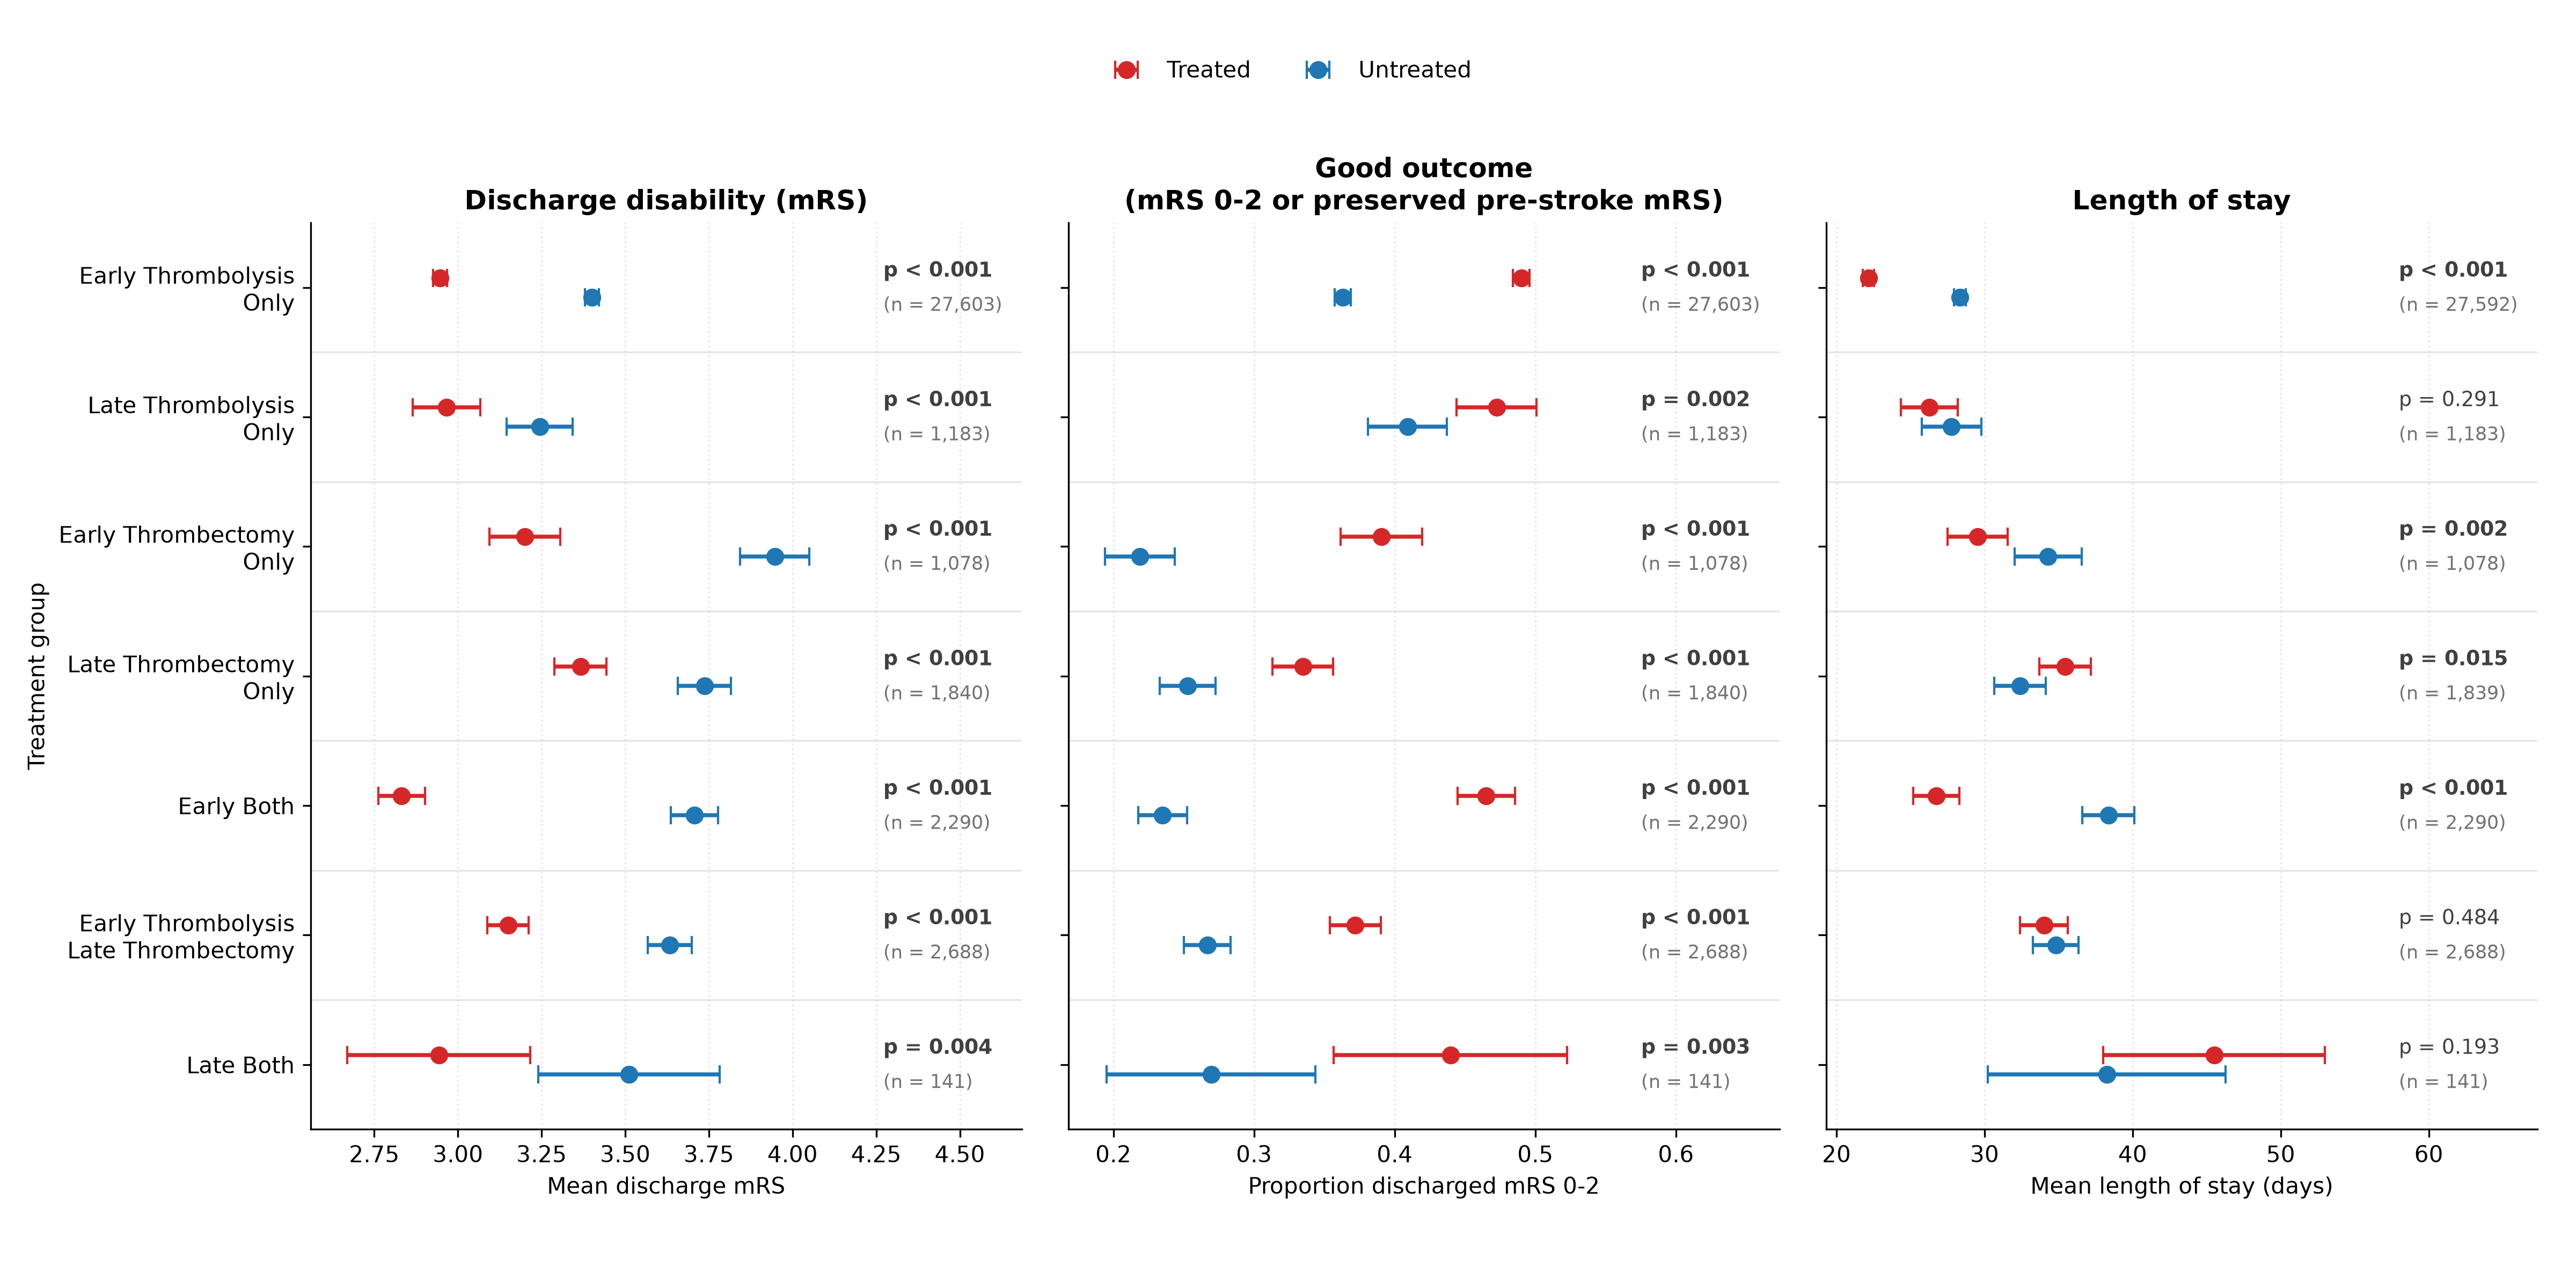
\includegraphics[width=1\linewidth]{images/non_mild_stroke_early_arrival_good_outcome_target_trial.png}
    \caption{Target trial emulation of reperfusion-treatment timing strategies and discharge functional outcomes, using matched control and treated patients. Estimated mean discharge modified Rankin Scale (mRS; left panel), proportion achieving an outcome of mRS 0–2 (middle panel), and length of stay (right panel) are shown for patients receiving each treatment strategy (red) and their matched untreated comparators (blue). Strategies are defined by early ($\leq$ 270 mins from onset) or late ($>$ 270 mins from onset) intravenous thrombolysis, mechanical thrombectomy, or their combination. Points denote estimated outcomes and horizontal bars 95\% confidence intervals; p-values indicate the treated–untreated comparison within each treatment group, with sample sizes shown. Lower mRS and higher mRS 0–2 proportions indicate more favourable outcomes.}
    \label{fig:main_target_trial_mrs_2}
\end{figure}